\section{Experimental Setup}
\label{sec:experiment}
%\KZ{Check the headings of all tables and figures. There are some inconsistencies in format and styles!}
This section describes the chatbots that we experiment with, the
set of baseline approaches that are compared to ChatMatch, and some
implementation details used in the following experiments.~\footnote{Data and source code are
released at: \url{https://github.com/ruolanyang/ChatMatch}.}

\subsection{Description of Seven Bots}
%\KZ{Put these and the next section into two tables to save space?} 
We pick seven chitchat chatbots trained or fine-tuned on ConvAI2 \citep{dinan2019second} to be evaluated in our experiments 
as \tabref{tab:bots} shows.
All chatbots are running and evaluated on a Intel (R) Xeon (R) CPU 
E5-2678 v3 @ 2.50GHz with NVIDIA GeForce RTX 2080 and a 12GB RAM. 

\begin{table}[th]
\centering
\small
%\scriptsize
\begin{tabular}{p{0.05\columnwidth}|p{0.85\columnwidth}}
%\hline
\toprule
\textbf{Bot} & \textbf{Description} \\ \midrule
BB & Blender Bot \citep{roller-etal-2021-recipes} is a
90M-parameter generative model following the training
of \citet{shuster-etal-2020-dialogue} and then finetuned on
blended skill talk tasks \cite{smith-etal-2020-put}.\\ \hline
 PL & PLATO-2 \citep{bao-etal-2021-plato} is a high-quality open-domain chatbot trained via curriculum learning.\\ \hline
 CS & A Seq2Seq model with Control.  \citep{see-etal-2019-makes} Here, we use their
specificity-controlled WD model (with WD repetition control).\\ \hline
%provided in this paper.
CR & The response-relatedness WD model
(with WD repetition control) provided in the paper about
Controllable Seq2Seq. \citep{see-etal-2019-makes} \\ \hline
UG & A large pre-trained seq2seq Transformer
with vocab unlikelihood which sets parameter
$\alpha = 100$ \citep{li-etal-2020-dont} \\ \hline
DG & DialoGPT medium. \citep{zhang-etal-2020-dialogpt}\\ \hline
 DD & Image Seq2Seq model. \citep{shuster-etal-2020-dialogue} \\
\bottomrule
\end{tabular}
\caption{Seven bots under evaluation(bot pool).}
\label{tab:bots}
\end{table}


%\begin{itemize}
%\item BB: Blender Bot \citep{roller2020recipes} which is a 
%90M-parameter generative model following the training 
%of \citet{shuster2020dialogue} and then finetuned on 
%blended skill talk tasks \cite{smith2020together}.
%\item PL: PLATO-2 \citep{bao2020plato}, a high-quality open-domain chatbot trained via curriculum learning.
%\item CS: A Seq2Seq model with Control.  \citep{see2019makes} Here, we use their 
%specificity-controlled WD model (with WD repetition control). 
%provided in this paper.
%\item CR: The response-relatedness WD model 
%(with WD repetition control) provided in the paper about 
%Controllable Seq2Seq. \citep{see2019makes}
%\item UG: A large pre-trained seq2seq Transformer
%with vocab unlikelihood which sets parameter 
%$\alpha = 100$ \citep{li-etal-2020-dont}
%\item DG: DialoGPT medium. \citep{zhang2020dialogpt}
%\item DD: Image Seq2Seq model. \citep{shuster-etal-2020-dialogue}
%\end{itemize}
 
\subsection{Baseline Evaluation Approaches}
We choose four automatic evaluation methods and one manual evaluation 
method to compete with CM. 
%Before applying these evaluation approaches on our 7 bots,
For the baselines which depend on static scripts,
we first make our seven bots 
generate responses for the 
%following
evaluation
using
the test set of DailyDialog \citep{li-etal-2017-dailydialog} 
as static scripts. 
%\KZ{Add how you apply these baselines on our 7 bots to get the eval
%results $\tau$. The first 4 are using the same test framework which is
%generate a response from a static script context. STB is human-bot. Ours is
%bot-bot.}
Then we apply the following baselines:

\noindent
\textit{PPL: Perplexity} 
Lower perplexity means that the generated sequence is 
more likely to be close to a human sentence.

\noindent 
\textit{TA: Token Accuracy}
Token Accuracy is used to measure the generation accuracy 
of each token, which refers to the ratio of the number of 
correctly predicted tokens to the total number of predicted tokens.


\noindent
\textit{BS: BERTScore}
We use a commonly used automatic evaluation metric for text generation, 
BERTScore from \citet{zhang2019bertscore}.
BERTScore
will return a similarity score between referenced answer and generated response
from the bot.
%computes a similarity score 

\noindent
\textit{HAE: Holistic and Automatic Evaluation} 
We combine the four separate metrics which measures Fluency, Context Coherence, 
Logical Self Consistency and Diversity from \citet{pang-etal-2020-towards} by distributing each bot a per-metric score(1-7)first and then summing them up to get a final score. 

\noindent
\textit{STB: Spot The Bot} 
The recently proposed interactive manual evaluation metric \textit{Spot The Bot} \citep{deriu-etal-2020-spot} asks human judges to decide whether the speaker is human or bot with a mix of human-bot and bot-bot chat logs.   
%We cut the dialogue logs into segments for every 2, 3, 5 exchanges, 
%and distribute them to human judges. It is up to human judges to decide 
%whether the chat is between humans, bots or unsure for each exchange. 
%The scores for being recognised as human is larger than that as unsure and then as a bot. Finally, the dominant round will 
%accumulate scores for the corresponding chatbot. 

%We also choose the recent proposed interactive manual evaluation metric  \textit{Spot The Bot} \citep{deriu-etal-2020-spot} as our baseline. In order to reproduce their evaluation %approach in a more simple way, we ask three college students who are skilled in English to be our annotators. We mix up our generated bot2bot chat logs with some human-bot %conversations and then cut them into short segments. Next, our annotators will give each turn a label which tells if the speaker is a bot from their prospectives. 


\subsection{Ground Truth for Rankings}
In order to obtain rankings that can be reliably used as ground truth, 
we asked a group of human judges who are fluent in English to chat 
with each of the seven bots and then manually assess the ability of 
the bots. 
Seven dimensions, namely fluency, 
knowledge, proactivity, specificity, 
diversity, consistency, and relevance, 
are used to help them complete the ranking task 
which are rated on a 5-point Likert-scale. 
We trained the human judges by providing them one 
positive example and one negative example for each dimension,
 following the suggestions for improving the quality
of human evaluation 
provided by \citet{clark-etal-2021-thats}.
Each judge can decide to 
stop the conversation whenever they feel confident enough to score
on these seven dimensions. We set the minimum number of exchanges
to be 20.
For each dimension, four judges participate in ranking 
bots' corresponding ability.
After, we also ask four judges to provide their 
overall ranking based on their general impression.
%After finishing the chats with all seven bots,  
%each judge will provide their score for each dimension
% and also a general ranking  (known as HR) based on the overall impression.
More details are shown in \appref{sec:humanappend}.
%\KZ{How do u aggregate the scores from each judge?}

We use Kendall ranking correlation ($\tau$) to evaluate the agreement 
among human judges and also between evaluation approaches and 
general human judgment. 
In the rest of the paper,
$\tau_{i}$ and $\tau_{g}$ are used to denote \textit{inter-judge agreement} 
and \textit{correlation between ranking produced by methods and the ground-truth
ranking} respectively.  
\tabref{tab:inter} shows $\tau_i$ on individual dimension and overall ranking. 
We believe
human judgements 
on each dimension
are reliable enough
as all of them
are greater than
0.6.
%We observe that $\tau_i$ for Consistency and Knowledge are lower than 
%that for other dimensions.
% We find from their
%chat logs 
% that they tend to test these two abilities
% by asking questions. 
%Specifically, when evaluating bots' knowledgeability, 
%human judges come up with some factual questions 
%related to their conversation topic at the time.
%Due to the differences among their questions and 
%the limited coverage of the questions, 
%human judges score the bots differently on this dimension. 
%The same is true for consistency, which is tested by asking the same question twice and then checking if the answers are contradictory.     
% \KZ{Here we need to explain why some of the
%$\tau$ scores are not very high, e.g., Con, Kno and Spf. 
%Anything under 0.33 is consider not very correlated? Also why Overall
%is higher than most other $\tau$'s.}

\begin{table*}[ht!]
\centering
%\scriptsize
\small
\begin{tabular}{lcccccccc}
%\hline
\toprule
& Fluency& Knowledge& Proactivity& Specificity& Diversity& Consistency & Relevance & Overall \\ \midrule
$\tau_i$ & 0.60 &0.62 & 0.60&0.62 &0.62 &0.61 &0.61 & 0.63  \\
\bottomrule
\end{tabular}
\caption{Inter-judge agreement on seven different dimension as well as overall ranking.}
\label{tab:inter}
\end{table*}
 
Later, we will analyze different $\tau_g$ 
considering human overall rankings as ground-truth ranking.  


\subsection{Parameters Settings for CM}
These settings are determined by empirics.
\begin{itemize}
\item  Each game contains 100 exchanges (200 turns) of conversation
to ensure a sufficient length to evaluate the bots.
\item  The starting utterance is always set to
a daily routing sentence
since the players of our tournament are chitchat bots.
\item For each game, the weight for individual dimension to be equal. 
%\item For each match, a bot will gain 3, 1 or 0 points for a win, tie or lose.
\item Each tournament has 42 games (21 matches) 
in total. 
%\item As match level, a bot will gain 3, 1 and 0 point for a win, tie and lose.
\end{itemize}

%\begin{figure*}[th]
%\centering
%\includegraphics[width=0.7\textwidth]{macro.eps}
%\caption{Scoreboard (Macro) and Rankings of 6-bot Tournament by ChatMatch.}
%\label{fig:macro}
%\end{figure*}

\section{Results and Analysis}
\label{sec:main}
%\KZ{Rephrase: In this subsection, we will first present the evaluation results from our automatic metrics, other baselines and human evaluation. 
%Then we will analyze the agreement between all automatic evaluation results and human judgments. }
In this section, we first present the end-to-end results from our automatic framework 
and other baselines.
Then we show that CM can generalize to different set of bots by applying CM on any 4-bot combination
of the bot pool and check the results.
Finally, we analyze the design of the framework with ablation tests in detail.  
%\subsubsection*{ChatMatch Final results}
%As we can see,  BB scores the top in our scoring framework (both for micro and macro). 
%BB is a competitive bot as it aims at performing well in multiple chitchat test sets in different domains. 
%CS and CR come in second and third respectively. They score quite close to each other as they use the same fine-tuned baseline seq2seq model, which only differ in the 
%choice of specific parameters for some improvement in different aspects. 
%DG and DD score close to each other. UG is always losing the match and ranks at the bottom. 
%We can find an obvious difference between the scores of  
%''the loser'' and the other five bots.

\subsection{End-to-end Evaluation of 7 Bots}
We deploy the five baseline methods and our framework CM on the 7 chatbots.
For simplicity, we convert the raw scores to rankings from 1 to 7 (the lower
the better) by
each of these methods. \figref{fig:botranks} depicts these rankings,
along with human ranking (HR) as a reference.
%\textcolor{red}{add some explanation after adding BERTScore}
BB ranks the top among all by CM and HR. 
This is not surprising because BB is a well-known competitive bot 
that performs well in many chitchat test sets and in different domains. 
The general trends exhibited by CM and STB track the human 
evaluation more
closely, whereas the trends of TA and BS are almost the reverse of human judgment.  
PPL is a popular approach for evaluating the
fluency of generated utterances, 
which can only evaluate whether 
the sequence generated by the model is 
close to human language without considering the context.
It can only reflect a part of the ability of a chatbot. 
%TA reflects whether the generated response matches the ground truth of the dataset. As reasonable responses are not limited to ground truth itself,
% it is difficult to correctly evaluate the ability of the chatbot with static scripts. 
We also find that HAE tends to give a higher score to the shorter response, 
so BB and other bots that tend to generate longer sequences are not evaluated
properly.

%CS comes in second. CS and CR are two controllable neural text 
%generation models using conditional training and weighted decoding to control
%different attributes.
%Here, CS is designed for controlling specifity while CR aims at controlling response-relatedness.
%%CS performs quite well in our automatic assesment based on seven dimensions. 
%PL, CR, DD and UG score close to each other. 
%DG always loses the match and ranks at the bottom.
%  
%We can see that BB ranks the best in Human Rankings. As for two common automatic metrics PPL and TA, CR ranks the best in PPL while UG and DD rank the best in TA. 
%BB and PL perform badly according to TA, which is inconsistent with our human evaluation results. 
%\KZ{Need more explanations about why we got these automatic results.
%And compared to human, discuss a bit...}

%\begin{table}[ht!]
%\centering
%\scriptsize
%%\small
%\begin{tabular}{lrrrrrrr}
%%\hline
%\toprule
%& BB &PL& CS & CR & UG & DG & DD  \\ \midrule
%PPL & 13.89 &11.64 &10.83 &\textbf{10.74} &16.35 & 20.19 & 14.88  \\
%TA & 0.12 & 0.05& 0.12& 0.10 & \textbf{0.23} & 0.19& \textbf{0.23}  \\
%HAE& 20 &\textbf{10} &11  &15 &11  & 24 & 21  \\ 
%STB & 2 &\textbf{1} &3 & 7& 6 & 5 & 4\\
%CM &\textbf{16}  &8&  15&7 &6& 0& 7\\\midrule
%%Micro & \textbf{58}&33 &42 &37 &39 & 25 & 34\\ 
%%CMR&\textbf{1} &3&2 &4 &6 &7 &4 \\ 
%Human& \textbf{1} &2& 4& 5& 7&6 & 3\\
%\bottomrule
%\end{tabular}
%\caption{Raw scores given by competing evaluation methods including
%human evaluation (best is
%bold in each row) \KZ{Include raw scores for STB and HR}.}
%\label{tab:baseline-scoring}
%\end{table}

\begin{figure}[th]
\centering
\includegraphics[width=\columnwidth]{rank3.eps}
\caption{Rankings of seven bots by different methods
%\textcolor{red}{Two of the reviewers complain that they don’t think a line graph is appropriate for Figure 3.}
}
\label{fig:botranks}
\end{figure}


\begin{table}[th]
\centering
\small
%\scriptsize
\begin{tabular}{lccc}
\toprule
Evaluation Type & Method & $\tau_{g}$ & Evaluation Time \\ \midrule
\multirow{4}{*}{Static Scripts}&PPL  &0.14 & \textasciitilde 30 secs \\
&TA&-0.35 & \textasciitilde 10 secs \\
&BS& -0.43 & \textasciitilde 10secs\\
&HAE&0.10 &\textasciitilde 2 min\\  \midrule
Human-bot  &STB &0.71 & \textasciitilde 60 min/human\\ 
\& bot-bot & & & \\
\midrule
Human-bot &HR &-  & \textasciitilde 90 min/human \\  \midrule
Bot-bot &CM& \textbf{0.81} & 2 min 57 secs\\
 \bottomrule
\end{tabular}
\caption{Correlation between ranking produced by different approaches and the ground-truth ranking 
and their respective evaluating time.}
\label{tab:main}
\end{table}

We further compute $\tau_g$ of the baselines and 
ours against the human rankings and include them in \tabref{tab:main}. 
%However, common automatic evaluation metrics such as PPL and HAE present poor agreements 
%with human judgments as their ranking agreement coefficient is close to zero, 
%which indicates a weak agreement. 
%TA is even negatively correlated with human judges. It  reflects whether the generated response matches the ground truth of the dataset. As reasonable responses are not limited to ground truth itself,
% it is difficult to correctly evaluate the ability of the chatbot with static scripts. 
%\textit{Spot The Bot} correlates well with human judgements as they 
%mainly depend on human annotations themselves.
The correlation between our metric and human judgment is 0.81,
% which is even better than the agreement among human judges ( $\tau_i = 0.53$ ). 
This indicates that CM's evaluation results 
are very close to the average 
judgment made by four different human judges. 

\textit{Spot The Bot} correlates well with human judgments as they
depend on human annotations themselves. 
However, common automatic evaluation metrics such as PPL and HAE 
present poor agreements with human judgments. 
TA, which assesses whether the 
generated response matches the ground truth
of the dataset, is even negatively correlated with human judges. 
%TA assesses 
%whether the generated response matches the ground truth 
%of the dataset. 
The same goes for BS, 
which computes token similarity with contextual embeddings.
Since there may be many other plausible responses than
the reference response itself, it is difficult to correctly evaluate 
the ability of the chatbot with static scripts.

\subsection{Time Efficiency}
\label{sec:time}
The efficiency of the competing methods is also assessed in \tabref{tab:main}. 
Though slower than other automatic methods,
CM is much faster than methods requiring human efforts. 
It takes a human judge 90 minutes on average to complete
the conversations with all 7 bots, decide ratings on seven dimensions and 
then give their overall ranking.
To put it in perspective, we ask three human judges to evaluate the same
7 bots by \textit{Spot The Bot} framework. It takes on average one hour for
each human judge to complete the ranking.

%We also notice a good correlation between ChatMatch's micro scoring metric
%and human judges on Non-repetitiveness dimension as 
%well. However, neither of our two scores fare very well with
%consistency, probably because it is harder for us to 
%detect implicit inconsistencies using our rules while human can better pick up such inconsistencies.

\subsection{Generalizability of ChatMatch Framework}
\label{sec:four}
To justify that CM framework works for different sets of bots,
we construct $\tbinom{7}{4} = 35$ test groups each of which consists of four randomly
chosen bots from our bot pool.
% ground truth ranking for each combination 
%of bots from human judgment. 
%To ensure the reliability of human judges,
%we only keep the groups whose inter-judge agreement is 
%higher than the average of all 35 test groups, which is 
%0.53.
%Then we have 17 four-bot groups left
Next, we implement the double-round CM on
these test groups.
Among 35 test groups, we found $\tau_g$ of 29 test groups are higher than 0.60 while the average $\tau_g$ equals
0.73. 
This indicates that CM is capable
of producing reliable rankings regardless
of the number and the combination of
participating bots.
\tabref{tab:fullfour} shows the full results of our generalizability tests. 
%As we can see, $\tau_g$ of 29 out of 35 groups is higher than 0.60.
We can tell that our framework is capable of predicting rankings for most of the combinations of bots. 
However, for a group of bots whose capabilities are relatively close, on which is even difficult for humans to reach an agreement(with $\tau_i$ relatively low in \tabref{tab:fullfour}), it is still difficult for our framework to rank them
accurately. 
Some of the chatlogs among these difficult bots are shown in \figref{fig:fourconvs}. Developing more precise metrics will be our next step work. 
%We present all results of 35 test groups in \appref{sec:general}.
%\KZ{rephrase this: Besides, we calculate the average agreement
%%% of these bot groups by using relative four-bot rankings deduced from original CM 
%results, which equals 0.68.
%As the values of the two average agreements are quite close, 
%it is convincing to believe that this evaluation framework
%presents good  generalizability.}
\begin{table*}[ht!]
\centering
%\scriptsize
\small
\begin{tabular}{lcclcc}
%\hline
\toprule
Combination of bots & $\tau_{g}$ & $\tau_{i}$ & Combination of bots & $\tau_{g}$ & $\tau_{i}$ \\ \midrule
BB, CR, CS, PL & 1.00 &0.61 & CR, DD, DG, UG & 0.67 & 0.60   \\
CR, CS, DG, PL & 1.00 & 0.78 & BB, CR, DD, PL & 0.67 & 0.70 \\
BB, CR, DG, PL & 1.00 & 0.72 & DD, DG, PL, UG & 0.67 & 0.61\\
BB, CS, DG, UG & 1.00 & 0.83 & BB, CS, DD, PL & 0.67 & 0.70 \\
BB, CS, DG, PL & 1.00 & 0.70 & CS, DD, DG, UG & 0.67 & 0.78\\
BB, DG, PL, UG & 1.00 & 0.89 & CR, DD, DG, PL & 0.67 & 0.61\\
BB, DD, PL, UG & 1.00 & 0.60 & CS, DG, PL, UG & 0.67 & 0.60\\
BB, DD, DG, UG & 1.00 & 0.67 & CS, DD, PL, UG & 0.67 & 0.61\\
BB, CR, CS, UG & 1.00 &0.96  & CR, DG, PL, UG & 0.67 & 0.60 \\
BB, CR, CS, DG & 1.00 & 0.78 & BB, CS, DD, DG & 0.67 & 0.61 \\
BB, CR, PL, UG & 1.00 & 0.76 & BB, CR, DD, DG & 0.67 & 0.67 \\
BB, CS, PL, UG & 1.00 & 0.76 & CR, DD, PL, UG & 0.55 & 0.61\\
CR, CS, PL, UG & 1.00 &0.61  & CR, CS, DD, UG & 0.33 & 0.61   \\
CR, CS, DG, UG & 0.67 & 0.61 & CS, DD, DG, PL & 0.33 & 0.61 \\
BB, CR, DG, UG & 0.67 & 0.61 & CR, CS, DD, DG & 0.33 & 0.61\\
BB, CR, DD, UG & 0.67 & 0.67 & BB, CR, CS, DD & 0.33 & 0.61\\
BB, CS, DD, UG & 0.67 & 0.61 & CR, CS, DD, PL & 0.0 & 0.61\\
BB, DD, DG, PL & 0.67 & 0.70 & & & \\
%CR, DD, DG, UG & 0.67 & 0.60 \\
%BB, CR, DD, PL & 0.67 & 0.70 \\
%DD, DG, PL, UG & 0.67 & 0.61 \\
%BB, CS, DD, PL & 0.67 & 0.70 \\
%CS, DD, DG, UG & 0.67 & 0.78 \\
%CR, DD, DG, PL & 0.67 & 0.61 \\
%CS, DG, PL, UG & 0.67 & 0.60 \\
%CS, DD, PL, UG & 0.67 & 0.61 \\
%CR, DG, PL, UG & 0.67 & 0.60 \\
%BB, CS, DD, DG & 0.67 & 0.61 \\
%BB, CR, DD, DG & 0.67 & 0.67 \\
%CR, DD, PL, UG & 0.55 & 0.61 \\
%CR, CS, DD, UG & 0.33 & 0.61 \\
%CS, DD, DG, PL & 0.33 & 0.61 \\
%CR, CS, DD, DG & 0.33 & 0.61 \\
%BB, CR, CS, DD & 0.33 & 0.61 \\
%CR, CS, DD, PL & 0.0 & 0.61 \\


%BB, DD, PL, UG & 0.33 & 0.59 \\
%CD, CR, DD, DG & 0.33 \\
%... & ... & ...\\  
\midrule
Average &  & & &0.73 &0.68  \\
\bottomrule
\end{tabular}
\caption{Full results for justifying the generalizability of CM.}
%\KZ{Maybe delete the last row with tau=0.33?}}
\label{tab:fullfour}
\end{table*}
  
%\textcolor{red}{explain 0.48, add one column for human inter-agreement}
%Then we implement CM on this test set and the rankings are shown in \tabref{tab:four}.
%\begin{table}[ht!]
%\centering
%\scriptsize
%\small
%\begin{tabular}{lrr}

%\toprule
%Combination of bots & $\tau_{g}$ & $\tau_{i}$ \\ \midrule
%BB, CR, CS, UG & 1.00 &0.95   \\
%BB, CR, CS, PL & 1.00 &0.61   \\
%CR, CS, PL, UG & 1.00 &0.61     \\
%BB, CR, DD, PL & 0.67 & 0.71 \\
%BB, DD, PL, UG & 0.33 & 0.59 \\
%CD, CR, DD, DG & 0.33 \\
%... & ... & ...\\  \midrule
%Average & 0.73 & 0.68 \\
%\bottomrule
%\end{tabular}
%\caption{Ranking for four randomly chosen bots 
%with CM. CM7 denotes the ranking of these four bots 
%through our original tournament. CM4 denotes the result
%from CM only
%using chat logs among the four chosen bots.
%Human denotes the human evaluation results. 
%}
%\caption{The Generalizability of CM.} 
%\KZ{Maybe delete the last row with tau=0.33?}}
%\label{tab:four}
%\end{table}

%Even if we only used the chat logs of four bots for the experiment, 
%the ranking does not change, which indicates that CM's output is 
%stable enough.


\subsection{Ablation Studies}
\label{sec:ablation}
The ChatMatch framework essentially consists of two main components: i) the 
bot-bot chat tournament set-up, and ii) the scoring metrics. 
Given its success in the end-to-end experiments,
one natural question to ask is whether the high correlation with the human
evaluation comes from the bot-bot set-up or the seven scoring metrics.
If the scoring metrics are significant, which ones are more useful?
In this subsection, we seek to answer these questions 
and also explore other factors or parameters in
CM that might contribute to its effectiveness, 
such as the number of exchanges 
%, similarity functions, 
and starting utterance.


\subsubsection{Effect of Different Chatting Setups}
We design two alternative settings to compete with our bot-bot tournament 
framework:

\noindent
\textit{Human-bot conversations}: we use our seven metrics to evaluate
the human-bot chat logs
collected 
from our human judges who
chat with bots directly. 
For each bot, we obtain the per-metric rankings (1-7) 
first and then we sum up the 7 per-metric rankings
for each bot
 to get their overall scores.
The final ranking is decided by the overall scores.
%Bots are ranked by this overall score in the end.

\noindent
\textit{Self-chat conversations}: 
we use our seven metrics to evaluate
the generated
 100-exchange self-chat logs 
and obtain the final rankings. 
The scoring process is similar 
to what we have done for the human-bot chat logs above.

As the results in \tabref{tab:frame} show, CM gets the highest agreement
 among the three frameworks while
implementing seven metrics 
on self-chat logs 
correlates weakly
to human judgments.
To figure out why our seven metrics do not 
work well with Human-bot setup and Self-chat setup, 
we calculate the average number of inconsistencies and relevant concepts
caught by our metrics, regardless of the speaker.
 We can tell from \tabref{tab:frame} that
Inconsistency is hardly
detected in Self-chat logs
as bots tend to chat about the same things
within this setup.
This can also explain why relevant 
concepts are often popular in self chat logs.
Under this 
circumstance, 
these two metrics are not 
capable of distinguishing bots' real
abilities.
 
Evaluating relevance with our metric
is difficult on human-bot logs. Human judges
are often switching topics by raising 
some questions to shorten the evaluation time.
That is why we are not able to evaluate bots'
ability for memorizing some long-distance concepts.
 
%Self-chat conversations do not seem natural 
%as we observe 70 repetitive turns
% for one 100-exchange self-chat conversation
%on average.
%Human-bot conversations are stronger than self-chat conversations
%as the quality of self-chat chat logs are poorer. 
%Human-bot conversations are chat logs from our ten human judges who
%chat with bots directly.
% which contains 21 exchanges on average per conversation.
%We normalize the number of inconsistencies and relevance to one hundred rounds
%to make a more reasonable comparison.
    
%\KZ{Any other take-ways?}
\begin{table}[ht!]
\centering
%\scriptsize
\small
%\begin{tabular}{lrrrrrrrr}
\begin{tabular}{lcccc}
%\hline
\toprule
Setup& $\tau_{g}$  & Inconsistency & Relevance &$l$   \\ \midrule
Human-bot& 0.29   &4.59& 0.88 &21   \\
Self-chat& 0.24  & 0.14 & \textbf{17.14} & 100\\
Bot-bot& \textbf{0.81}  & \textbf{7.10} & 12.60&100 \\
%TS& & & &\\
%Top bot &BB &PL &BB &BB &BB &UG &UG\\
\bottomrule
\end{tabular}
\caption{
%Average score on
%individual dimension
%and 
%agreement (kendall's $\tau$) with human judges 
%for different setup.
Effects of different chat setups using the same scoring metrics. 
%Here, human-bot conversations are chat logs from our ten human judges who
%chat with bots directly.
$l$ refers to the number of exchanges.
 %\KZ{This table is problematic.
%the negative correlations are hard to explain. The explainable
%in the text below is not convincing.}
}
\label{tab:frame}
\end{table} 

%\begin{table}[ht!]
%\centering
%\scriptsize
%\small
%\begin{tabular}{lrrrrrrrr}
%\hline
%\toprule
%Setup&$\tau_F$& $\tau_K$& $\tau_P$& $\tau_S$& $\tau_D$& $\tau_C$ &$\tau_R$ &$\tau_g$ \\ \midrule
%HB &0.42 &0.50 &0.68 &-0.05 &0.74 &-0.53 &-0.70 &0.29 \\
%SC &0.05 &0.12 &0.10 &-0.20  &0.55 &0.01 &0.49 & 0.24  \\
%CM &0.53 &0.05 &0.29 &0.29  &0.59 &0.05 &0.49 & 0.81\\ 
%Top bot &BB &PL &BB &BB &BB &UG &UG\\
%\bottomrule
%\end{tabular}
%\caption{Effects of different
%chat setups on each individual metric
%and their combination.
%\KZ{This table is problematic.
%the negative correlations are hard to explain. The explainable
%in the text below is not convincing.}
%}
%\label{tab:metric}
%\end{table}

 
%\begin{table}[th!]
%\centering
%\small
%\begin{tabular}{lr}
%\hline
%\toprule
%Chat Setup& Agreement ($\tau$)\\ \midrule
%Human-bot   & 0.39  \\
%Self-chat  & 0.30  \\
%Bot-bot tounament(CM)  & \textbf{0.68}  \\
%\bottomrule
%\end{tabular}
%\caption{
%Agreement (kendall's $\tau$) with human judges for different framework 
%}
%\label{tab:frame}
%\end{table}


\subsubsection{Effect of different scoring metrics}
To understand the role and effects of each
scoring dimension at game level, 
each time we set one dimension coefficient to zero
and others remain one. We call these experiments
``minus $x$" experiments where $x$ is one of the 
metrics under testing.  
\tabref{tab:minus} shows the agreement with human judges 
that comes from each ``minus $x$" experiment. 

%\KZ{I think we need the results of all - x, where x is one of the
%7 metrics.}

\begin{table*}[ht!]
\centering
%\scriptsize
\small
\begin{tabular}{lcccccccc}
%\hline
\toprule
&- Fluency&-Knowledge& -Proactivity& -Specificity& -Diversity& -Consistency & -Relevance &All \\ \midrule
%$\tau_i$ & & & & & & & \\
$\tau_{g}$ &0.62 &0.71 &0.71&0.62 &0.24&0.71& 0.71&0.81   \\
%Top bot &BB &PL &BB &BB &BB &UG &UG\\
\bottomrule
\end{tabular}
\caption{Correlation between ranking produced by CM while eliminating different scoring metrics and ground truth ranking.
%\KZ{This table is problematic.
%the negative correlations are hard to explain. The explainable
%in the text below is not convincing.}
}
\label{tab:minus}
\end{table*}


%\begin{table}[ht!]
%\centering
%\scriptsize
%\small
%\begin{tabular}{lrrrrrrrr}
%\hline
%\toprule
%&Flu& Kno& Pro& Spf& Div& Con & Rel  \\ \midrule
%Human-bot &9.27 &0.29 &16.37&0.72 &2.37 &0.96& 0.19   \\
%Self-chat & 6.4 & 0.29 & 31.29 & 0.59 & 69.86 & 0.14 & 31.42\\
%CM & 10.35 & 0.33 & 30.69 & 0.64 & 68.15 & 7.10 & 12.60 \\
%Top bot &BB &PL &BB &BB &BB &UG &UG\\
%\bottomrule
%\end{tabular}
%\caption{

 %\KZ{This table is problematic.
%the negative correlations are hard to explain. The explainable
%in the text below is not convincing.}
%}
%\label{tab:count}
%\end{table}


%\begin{table}[ht!]
%\centering
%\small
%\begin{tabular}{lrrrr}
%\toprule
%& Average& STD& Min&Max \\ \midrule
%Flu & 4.12&0.62&3.39&4.76   \\
%Spf &0.65 &0.04 &0.58 &0.70\\
%\bottomrule
%\end{tabular}
%\caption{Average, Standard Deviation, Minimum and Maximum of Score for Fluency and 
%Specificity per turn among seven bots. 
%STD, Min and Max denote 
%the standard deviation, 
%minimum and maximum score
% for two dimensions respectively.
%}
%\label{tab:average}
%\end{table}

Eliminating any of the metrics presents an effect on evaluation as $\tau_g$ has dropped.
% \textcolor{green}{zitong:,showing
%the seven metrics we designed are meaningful and can help to evaluate the overall quality of the dialogue.}
However, removing diversity does the most harm to evaluation as $\tau_g$ has dropped from 0.81 to 0.24. 
That is because diversity is usually the first thing that comes to human judges' minds while doing the evaluation. 
Improving lexical diversity and reducing repetition are still major
challenges encountered by chat-bots developers.
%Eliminating Diversity and Relevance presented a strong effect on evaluation as $\tau_{g}$ has dropped from 0.68 to 0.05 and 0.20 respectively. 
%These two dimensions are usually the first two things that come to human judges' minds while completing the evaluation. Bots that generate highly context-related and diverse responses always rank highly in human evaluation.

%Removing Fluency, Specificity or Consistency has little effect on $\tau_{g}$. As for Consistency, we calculate the average number of inconsistency that we have caught 
%with our algorithm described in \algoref{algo:inconsist}, which is 7 per conversation with standard deviation equals 16. 
%Out of 42 conversations, no inconsistency was detected in 28 conversations. 
%However, this does not mean there is no inconsistency in these conversations.
%We ask two human annotators to annotate the inconsistency 
%for all chatlogs. 
%They finally find \textcolor{red}{insert a number} in total.
%Currently, CM is not able to detect implicit inconsistency which does not follow a question. 
%We also train a BERT \citep{devlin2018bert} classifier on Dialogue NLI dataset \citep{welleck2018dialogue}.
% Inconsistency detection is proceeding by considering contradiction predictions from the BERT NLI model to be inconsistency cases in a dialogue. 
%However, the average number of detected inconsistency is only 
%\textcolor{red}{insert a number}
%per conversation.  
%Developing a more potent inconsistency detection method
%that can make bots more likely to 
%expose their weakness on this dimension
% will be one of our future goals.


%As for Fluency and Specificity, 
%we calculate the average and 
%standard deviation 
%of these two scores
%among seven bots.
%Seven bots score 
%closely 
%at these two dimensions: 
%4.12 per turn on average for Fluency with standard deviation equals 0.62 
%and 0.65 for Specificity with standard deviation equals 0.04. This indicates that their ability at these two dimensions is quite close to each other so that canceling them will not have much impact on the final results.
%\begin{table}[ht!]
%\centering
%\small
%\scriptsize
%\begin{tabular}{lrrrr}
%\toprule
%& Average& STD& Min&Max \\ \midrule
%Flu & 4.12&0.62&3.39&4.76   \\
%Spf &0.65 &0.04 &0.58 &0.70\\
%\bottomrule
%\end{tabular}
%\caption{Average, Standard Deviation, Minimum and Maximum of Score for Fluency and
%Specificity per turn among seven bots.
%STD, Min and Max denote
%the standard deviation,
%minimum and maximum score
% for two dimensions respectively.
%}
%\label{tab:average}
%\end{table}
%Agreements between Specificity, Fluency, Proactivity and 
%human judgments are quite weak since 
%they have less influence on human evaluation 
%\KZ{I'm not sure about this. Any proof? The inter-judge agreement on Pro is quite high at 0.5!}, 
%even though they are important abilities for bots to improve.
%Knowledge and Consistency are weakly negatively correlated to human judgments. The first main reason for this is that they are often ignored by humans while ranking the bots. \KZ{That's why the low
%correlations among humans in \tabref{tab:inter}?} 
%Second, our automatic rule-based algorithms can only
%capture limited instances of inconsistency and ignorance. 
%This kind of inconsistency and ignorance are always common in less capable bots. \KZ{GIve some numbers here?} 
%More potent detection rules will be introduced in the future.

%\KZ{Add a table to show the average number of times each dimension
%is captured within 100 exchanges. This can explain some of the negative
%correlations or small $\tau$ numbers in other tables.}

Additionally, to compare our scoring metrics with other 
unsupervised metrics, we try to add the metrics including Fluency, Context Coherence, Logic Self Consistency and Diversity
from HAE \citep{pang-etal-2020-towards} 
into CM.
%Because these 4 metrics can be computed without reference utterances. 
%The authors does not provide a way to combine 
%the four metrics mentioned in the paper.
Since these four metrics are all reference-independent, we can test them with our bot-bot tournament framework. 
Results shown in \tabref{tab:met} indicate that
the four metrics do not work well with bot-bot settings and
%Not only the metrics designed by us can be used in our framework,
%but 
 metrics need to be carefully designed to suit bot-bot chatting.
%\textcolor{green}{zitong:
%This paragraph has been rewritten again at 15:22, please check.
%}

%This is because, in \tabref{tab:main}, the four metrics are trained on 
%DailyDialog and tested on static scripts from DailyDialog. 
%Therefore, while CM is a flexible framework that can accommodate more
%metrics, they need to be carefully designed to suit bot-bot chatting.
%HAE with bot-bot chat setup obtains a weaker agreement
%as every separate metric from HAE is trained on 
%DailyDialog.
% Consequently, we doubt that even if 
%HAE itself does not need
%any reference while implementing the 
%evaluation, it still relies a lot 
%on testing with DailyDialog.
%\KZ{Don't understand this table. Elaborate some more? HAE was an
%eval method, why is it a metric now?}
%\textcolor{red}{Need explain more?}
%\textcolor{green}{zitong:
%Deleted 1 paragraph.
%}

\begin{table}[th!]
\centering
%\scriptsize
\small
\begin{tabular}{lc}
%\hline
\toprule
Metric  & $\tau_{g}$\\ \midrule
CM (with HAE's metrics) & 0.14 \\
CM (with our metrics)  & \textbf{0.81}  \\
\bottomrule
\end{tabular}
\caption{
Comparison with CM using HAE's metrics.
}
\label{tab:met}
\end{table}


\subsubsection{Effect of the Starting Utterance}

As most of the chitchat bots we test in the competition 
are for open domain, we use three types of starting utterances, 
namely {\em greetings}, {\em declarative statements}, and 
{\em questions}. 
We show one example for each type in 
\tabref{tab:multi-context}.

\begin{table}[th!]
\centering
\small
%\scriptsize
\begin{tabular}{llc}
%\hline
\toprule
 & Example  & $\tau_{g}$\\ \midrule
Greetings  & ``Hi! How are you?'' & 0.62  \\
Declarative  & ``Not feeling well this morning.'' & 0.71  \\
Question  & ``What did you do last week? '' & \textbf{0.81}  \\
%Average  & & 0.35  \\
\bottomrule
\end{tabular}
\caption{
The effects of different starting utterances.} 
%Average denotes agreement after summing up scores with 
%three different starts.}
\label{tab:multi-context}
\end{table}

As \tabref{tab:multi-context} shows,
 all three starting utterances lead to a 
good correlation with human judgments. 
The model that starts with a question performs the best since 
raising a question is always a good way to start a conversation 
and make the bots start talking about it.
%However, we do not find a significant difference with different 
%starting utterance. 
We also find that when two 
bots are free to talk without human intervention, they prefer 
to steer the chat to their ``comfort zones'' (e.g., talking about 
their basic personal information) rather than stick to the ball 
``started'' by CM. 
Hence, we decide to use the question in other experiments.
%\KZ{In the end, do we use the questions only or a combination of
%all three? This is not said. Also, I think we should also
%test combination? If we use only questions to achieve 0.68 in the
%end to end tests, we should have said this in the experiment setup
%or approach?} 

\subsubsection{Number of Exchanges in a Game} 

We also test CM with a different number (e.g., 5, 10, 25, 50, 100, 150 and 200) of exchanges in a game.
A game of no less than 100 exchanges reaches the best agreement between 
CM and human judgments. As a result, we use 100 exchanges in other experiment, which we believe is long enough to make the bots
 expose their flaws
and show their strengths.
%\KZ{Add a graph here.}
\begin{figure}[th]
\centering
\includegraphics[width=\columnwidth]{number3.eps}
%\includegraphics[width=\columnwidth]{exchange.pdf}
\caption{Effects of number of exchanges per game.}
%\KZ{Rankings of seven bots by different methods, also fonts too small in figure%.x-label needs rephrasing.}}
\label{fig:number}
\end{figure}


%\subsubsection{Similarity Functions} 
%\KZ{This section can be cut.}
% We provide a set of simple similarity functions 
%to score diversity(non-repetitiveness) and consistency in chat logs which are: 
%tf-idf cosine similarity, mean of Word2Vec sentence cosine similarity 
%and Bag-of-Word Jaccard coefficient. $\tau_{g}$ using these three functions are 0.68, 0.65 and 0.62 respectively. We choose tf-idf cosine similarity in
%the rest of the experiments.

%\begin{table}
%\scriptsize
%\centering
%\begin{tabular}{lcccc}
%\toprule
%&tf-idf & Word2Vec & Jaccard \\ \midrule
%$\tau$ &\textbf{0.68} &  0.65 & 0.62\\
%Time &\textbf{ 2m 57s} &  3m 1s & 5m 52s\\ \bottomrule
%\end{tabular}
%\caption{Comparison of three similarity functions using $\tau$ agreement.}
%\KZ{Run a few times to get average timem then update the number in time efficiency section.}
%\label{tab:similarity}
%\end{table}  



%\subsubsection{Weights of Scoring Dimensions}
%\KZ{remove this subsubsection.}
%Here we test two sets of weights which are used for summing up 
%individual dimensions at game-level:
%\begin{itemize}
%\item Equal weights: each dimension is worth one point.
%\item Linear-combination weights: we fine-tune seven 
%coefficients with a linear regression model
% according to the scores on these seven dimensions 
%and the overall rankings provided by human judges, 
%we set $fluency = knowledge = diversity = 0.33$, others$=0$.
%\KZ{Why are other coefficients zero?}
%\end{itemize}

%The final results with alternative choices  are: 
%$\tau^i = 0.68, \tau^f = 0.14 $ respectively. 
%It is not surprising to find weak agreement between our framework with fine-tuned weights and human judgments as 
%humans' standards for individual dimension rating are usually rather ambiguous according to \tabref{tab:inter}. As a result, inter-agreement among human judges on individual dimension is quite weak and the parameters fine-tuned based on this relationship are no longer reliable.

%Since equal weight performs better, this setting is adopted in
%other parts of the experiments. 

 
\subsubsection{Different Ranking Methods}
%\textcolor{green}{zitong: In sports tournaments, there are also some scoring systems, from which we have got some inspiration. Although they are simpler than our method, we have experimented with them.}
Ranking is an inevitable part in sports competitions.
Hence, in addition to TrueSkill ranking system,
 we have tried two other ranking methods commonly used in
sports~\cite{wiki-sport-scoring}:
%, addition to in Trueskill 
\begin{itemize}
\item win = 3, tie = 1, lose = 0
\item win = 2, tie = 1, lose = 0
\end{itemize}

With these sets of parameters, 
 $\tau_g$ are both 0.62 while TrueSkill ranking setting correlates the best. 
%and used throughout
%the experiments.
%\textcolor{green}{zitong:
TrueSkill ranking is capable of describing the ability of each bot in a more detailed way with their distribution than simply accumulating the points.
%}
%\subsection{Time Efficiency}
%\label{sec:time}
%As for timing, a human judge takes more than 90 minutes on average to complete 
%the conversations with all 7 bots, decide ratings on seven dimensions and then rank the bots. 
%Our system only requires about 2 min 57 secs on average to 
%complete a game, 
%which is an 100-exchange conversation. As all 42 games can be processed in 
%parallel, the total time cost for evaluating all the 6 bots is less than
%3 minutes. To put it in perspective, when we evaluate the same
%6 bots by \textit{Spot The Bot} framework, it takes on average one hour for
%each human judge to complete the ranking.


\subsection{Variety in Bot-bot Chats}
\label{sec:diversity}
It is commonly thought that we evaluators have less control over
the bot-bot conversations than human-bot conversations as the automatic dialogue could veer into
any direction. 
However, this does not mean that bot-bot chat logs are all that bad in quality, 
or less useful for evaluation.
While going through bot-bot chat logs, 
we find that sometimes 
conversations between bots 
carry even more variety than that between human and bot. 
To demonstrate such serendipity, 
we present the average specificity score of the bot's utterances
in \tabref{tab:div} which indicates the variety of the use 
of words in dialogue.  

% \KZ{Why do we pick CR to evaluate this?
%Why chat with PL? These choices must be justified. Otherwise it's
%`` ad hoc''!} 
We can see that bots tend to generate longer 
responses while chatting with other bots. 
The diversity of words in bot-bot and human-bot conversations
 are quite close.
%\KZ{
%It is true that bot-bot conversations are less controllable 
%compared with human-bot conversations as we could not decide 
%the direction of the chat. 
More examples extracted from our collected
bot-bot chat logs are shown in \appref{sec:bot-bot chat}.
%}

\begin{table}[th]
%\scriptsize
\small
\centering
\begin{tabular}{lccccc}
\toprule
& D-1 & D-2 & avg(D-1, D-2)&Avg Len\\ \midrule
human-bot & 0.44  & \textbf{0.89}   &\textbf{0.67}  &12.8 \\ \midrule
bot-bot & \textbf{0.49}  &0.83    &0.66 &\textbf{15.7} \\ \bottomrule
\end{tabular}
\caption{Average Distinct-1/2 and average lengths of 
bot utterances in different types of chat logs. }
\label{tab:div}
\end{table}

%\subsection{Discussion}
%In our experiments, we only test chatbots used for daily chatting. 
%It would also be useful to test chatbots from other domains 
%(e.g., domain-specific bots with specialized knowledge, 
%empathetic bots used for entertainment, etc.) in the future.  
%In order to detect more subtle weakness in bots, we probably 
%need a more comprehensive setup for future design of the system . 

